\chapter{Campaign and Analysis}
\label{campaign_and_analysis}
The Analysis of this campaign bases of the observation campaign of NGC4593 in 2016 by Edward M. Cackett \parencite{cackett2018accretion}. The observations took place between the 12th of July and the 6th of August with 26 successful observations and was performed with the Hubble Space Telescope (HST) using the Space Telescope Imaging Spectrograph (STIS). The following section will cover important properties of NGC4593 and the 2016 campaign.

\section{NGC4593}
\label{NGC4593}

NGC4593 is an active galactic nuclei (AGN), classified as an Seyfert 1 Galaxy with a Sb D morphology.  It is located at RA = 12:39:39.44, DEC = -05:20:39.03 (2000) and has a of $ z = 0.0083 \pm 0.0005$ This correspond to a distance of about $35.6$ MPc \parencite{simbaNGC4593}based on the $\Lambda$CDM-Model. 

\begin{figure}[!ht]
	\centering
	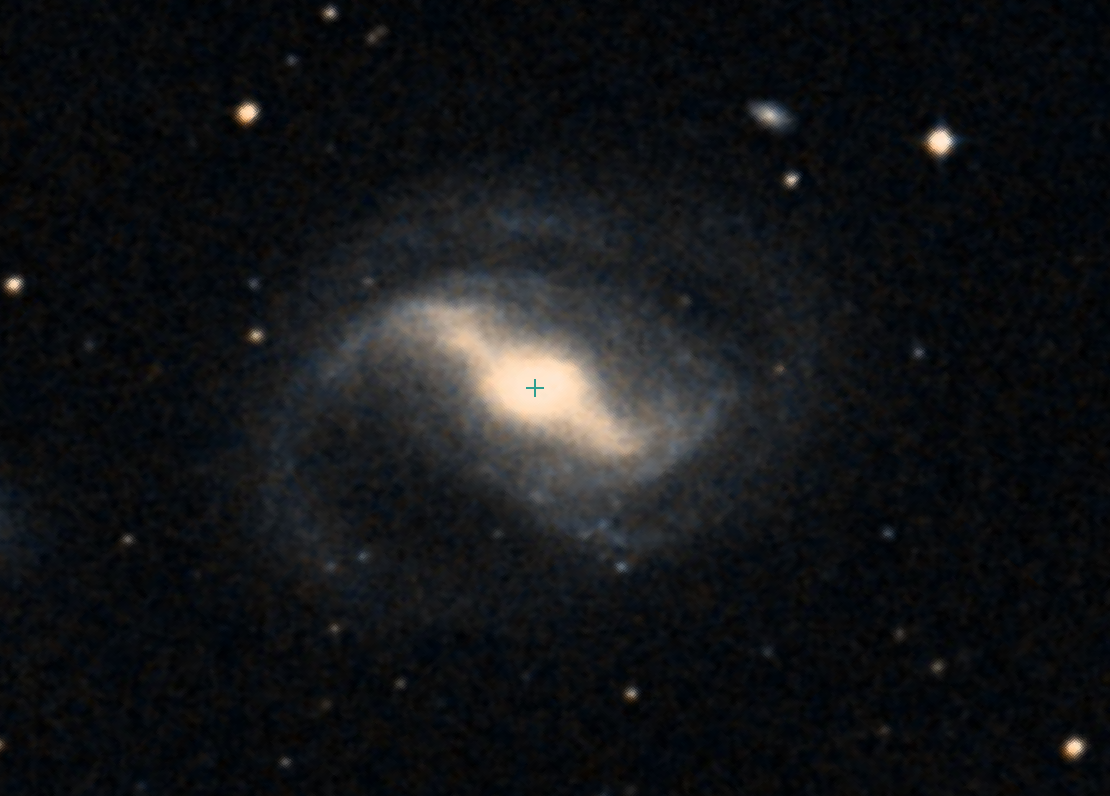
\includegraphics[width=0.5\textwidth]{pictures/Chapter2/NGC4593.PNG}
	\caption{A DSS image of NGC4593.}
	\label{fig:NGC4593}
\end{figure}

\section{2016 Campaign by E. M. Cackett}
\label{Campaign_Cackett}

E. M. Cackett's campaign was designed to study wavelength dependent continuum lags. Therefore, the STIS instrument on the Hubble Space Telescope was used with low-resolution gratings to measure a broad range of wavelengths. In each observation, spectra were taken using three different gratings: G140L, G430L, and G750L. These were used together with the $52'' \times 0.2''$ slit.\\
The characteristics of the STIS gratings used in this analysis are summarized in Table \ref{tab:stis_gratings}.

\begin{table}[h!]
	\centering
	\small
	\caption{Overview of STIS Grating Characteristics \parencite{stisgratings}}
	\label{tab:stis_gratings}
	\begin{tabular}{lcccc}
		\hline
		\textbf{Grating} & \textbf{Range [\AA]} & \textbf{Exp. Time [s]} & \textbf{Res. Power} & \textbf{Dispersion [\AA/pixel]} \\
		\hline
		G140L  & 1119--1715  & 1234 & $\sim 1000$         & 0.6 \\
		G430L  & 2888--5697  & 298  & $\sim 500 - 1000$    & 2.73 \\
		G750L  & 5245--10233 & 288  & $\sim 500 - 1000$    & 4.92 \\
		\hline
	\end{tabular}
\end{table}

